\section{DBMS e Linguaggi}
Si distinguono tre diversi livelli di descrizione dei dati:
\begin{itemize}
    \item A livello di \textcolor{purple}{\emph{vista} logica}: descrive come deve apparire il database a seconda dell'utente che lo usa, in base ai suoi permessi.
    \item A livello \textcolor{purple}{logico}: descrive la struttura degli insiemi dei dati e le relazioni fra essi,
        senza doversi occupare della loro organizzazione nella memoria.
    \item A livello \textcolor{purple}{fisico}: viene descritto come sono organizzati fisicamente i dati nella memoria e
        vengono riportate quali strutture dati ausiliare vengono utilizzate.
\end{itemize}

\begin{center}
    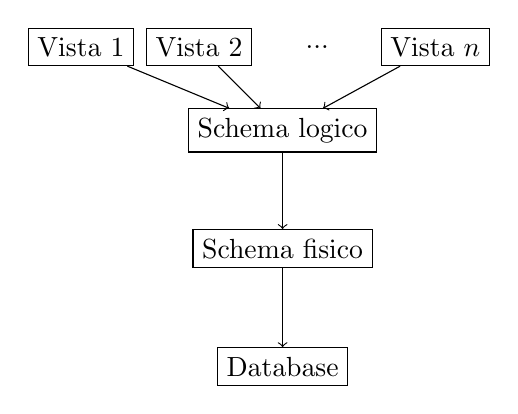
\begin{tikzpicture}[node distance = 1.5cm, main/.style={rectangle, draw}]
        \node[main] (1) {Vista 1};
        \node[main] (2) [right of=1] {Vista 2};
        \node[main, draw opacity=0] (3) [right of=2] {...};
        \node[main] (4) [right of=3] {Vista $n$};
        \node[main] (5) [below right of=2] {Schema logico};
        \node[main] (6) [below of=5] {Schema fisico};
        \node[main] (7) [below of=6] {Database};
        \draw[->] (1) -- (5);
        \draw[->] (2) -- (5);
        \draw[->] (4) -- (5);
        \draw[->] (5) -- (6);
        \draw[->] (6) -- (7);
    \end{tikzpicture}
\end{center}

Quest approccio permette di garantire le proprietà di indipendenza logica e fisica:
\begin{itemize}
    \item \textbf{\textcolor{purple}{Indipendenza Logica}}: gli applicativi non necessitano modifiche in seguite a variazioni dello schema logico.
    \item \textbf{\textcolor{purple}{Indipendenza Fisica}}: gli applicativi non necessitano modifiche in seguito a cambiamenti dell'organizzazione fisica dei dati.
\end{itemize}

Per quanto riguarda i linguaggi di interrogazione, questi possono essere distinti in:
\begin{itemize}
    \item \textbf{\textcolor{purple}{DML}} (Data Manipulation Language): per l'interrogazione e l'aggiornamento dei dati.
    \item \textbf{\textcolor{purple}{DDL}} (Data Definition Language): per la definizione di schemi, sia logici che fisici, ed altre operazioni. 
\end{itemize}

\subsection{Funzionalità del DBMS}
Un DBMS deve prevedere più modalità d'uso per soddisfare le esigenze di più categorie di utenti
che accedono al database. Deve poter offrire:

\begin{itemize}
    \item Un'interfaccia grafica per accedere ai dati.
    \item Un linguaggio di interrogazione per gli utenti inesperti (non programmatori).
    \item Un linguaggio di programmazione per chi sviluppa applicazioni, nello specifico deve prevedere
        l'integrazione del \emph{DDL} e del \emph{DML} nel linguaggio ospite.
    \item Un linguaggio per lo sviluppo di interfacce per le applicazioni.
    \item Predisporre per l'\textcolor{purple}{amministratore} strumenti per stabilire i diritti d'accesso ai dati,
        per il ripristino del sistema e per la modifica e la definizione degli schemi logici (sia interno che esterno).
    
\end{itemize}

\subsection{Proprietà dei Database}
Il DBMS permette di garantire al database le seguenti proprietà:
\begin{itemize}
    \item \textcolor{purple}{Integrità}: mantenimento dei vincoli d'integrità dichiarati in fase di definizione dello schema.
    \item \textcolor{purple}{Affidabilità}: protezione dei dati da parte di malfunzionamenti sia software che hardware e da anomalie indesiderate
        come l'accesso concorrente al database da parte di più utenti.
    \item \textcolor{purple}{Sicurezza}: protezione dei dati da parte di utenti non autorizzati.
\end{itemize}

Inoltre un DBMS deve essere in grado di gestire collezioni di dati che siano:
\begin{itemize}
    \item \textcolor{purple}{Grandi}
    \item \textcolor{purple}{Persistenti}: il periodo di vita dei dati è indipendente dai programmi che li utilizzano.
    \item \textcolor{purple}{Condivise}: possono essere usati da programmi diversi.
\end{itemize}

Il DMBS deve essere anche \textcolor{purple}{efficiente} (utilizzando al meglio le risorse in termini di \emph{spazio} e \emph{tempo}) ed \textcolor{purple}{efficace}.

\subsection{Transazioni}

\begin{definition}[Transazione]
    Una transazione è una serie di azioni di lettura e scrittura sulla memoria permanente
    o di elaborazione dati in memoria temporanea. Presenta le seguenti proprietà:
    \begin{itemize}
        \item \textbf{\textcolor{purple}{Atomicità}}: le transizioni che non vanno a buon fine o che vengono abortite
            sono trattate come se non fossero mai state eseguite.
        \item \textbf{\textcolor{purple}{Persistenza}}: le modifiche effettuate da una transizione andata a buon fine sono permanenti,
            ovvero non possono essere alterate da malfunzionamenti.
        \item \textbf{\textcolor{purple}{Serializzabilità}}: nel caso di esecuzioni concorrenti di più transazioni, l'effetto ottenuto è quello di un'esecuzione seriale.
    \end{itemize}
\end{definition}

\section{Modellazione}
\begin{definition}[Modello Astratto]
    Un modello astratto è la rappresentazione formale di idee e conoscenze relative ad un fenomeno.
\end{definition}

La modellazione è centrale nella progettazione del database che comprende le fasi presenti in figura.
\begin{center}
    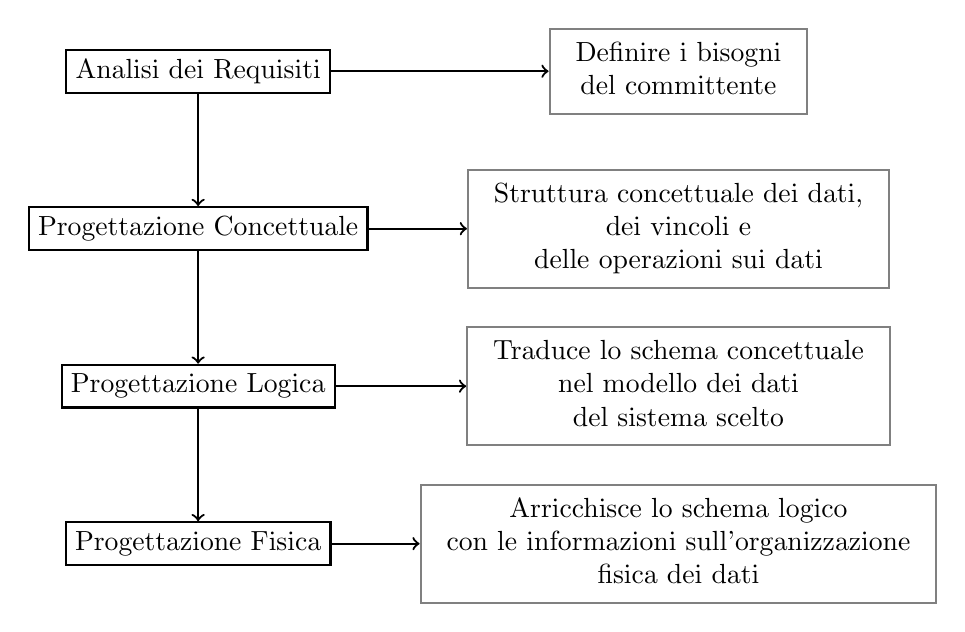
\begin{tikzpicture}[thick, main/.style = {draw, rectangle}, desc/.style = {draw=gray, rectangle}]
        \node[main] (1)  {Analisi dei Requisiti};
        \node[main] (2) [below of=1, node distance = 2cm] {Progettazione Concettuale};
        \node[main] (3) [below of=2, node distance = 2cm] {Progettazione Logica}; 
        \node[main] (4) [below of=3, node distance = 2cm] {Progettazione Fisica};
        \node[desc] (5) [right of=1, node distance = 6.1cm] {\begin{tabular}{c} Definire i bisogni \\ del committente \end{tabular}};
        \node[desc] (6) [below of=5, node distance = 2cm] {\begin{tabular}{c} Struttura concettuale dei dati, \\ dei vincoli e \\ delle operazioni sui dati \end{tabular}};
        \node[desc] (7) [below of=6, node distance = 2cm] {\begin{tabular}{c} Traduce lo schema concettuale \\ nel modello dei dati \\ del sistema scelto \end{tabular}};
        \node[desc] (8) [below of=7, node distance = 2cm] {\begin{tabular}{c} Arricchisce lo schema logico \\ con le informazioni sull'organizzazione \\ fisica dei dati \end{tabular}};
        \draw[->] (1) -- (2);
        \draw[->] (2) -- (3);
        \draw[->] (3) -- (4);
        \draw[->] (1) -- (5);
        \draw[->] (2) -- (6);
        \draw[->] (3) -- (7);
        \draw[->] (4) -- (8);
    \end{tikzpicture}
\end{center}

\subsection{Fasi della Modellazione}

\begin{center}
    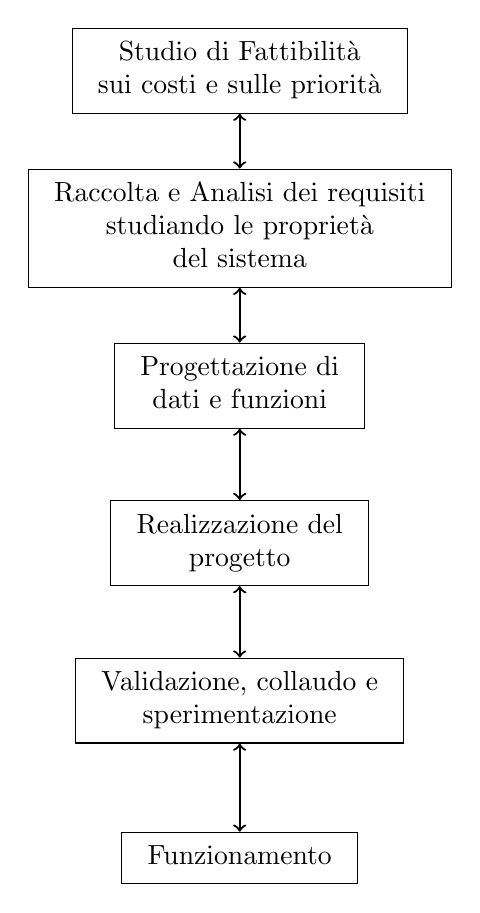
\begin{tikzpicture}[node distance=2cm, main/.style={draw, rectangle}]
        \node[main] (1) {\begin{tabular}{c}Studio di Fattibilità \\ sui costi e sulle priorità\end{tabular}};
        \node[main] (2) [below of=1] {\begin{tabular}{c}Raccolta e Analisi dei requisiti \\ studiando le proprietà \\ del sistema\end{tabular}};
        \node[main] (3) [below of=2] {\begin{tabular}{c}Progettazione di \\ dati e funzioni\end{tabular}};
        \node[main] (4) [below of=3] {\begin{tabular}{c}Realizzazione del \\ progetto\end{tabular}};
        \node[main] (5) [below of=4] {\begin{tabular}{c}Validazione, collaudo e \\ sperimentazione\end{tabular}};
        \node[main] (6) [below of=5] {\begin{tabular}{c}Funzionamento\end{tabular}};
        \draw[<->, thick] (1) -- (2);
        \draw[<->, thick] (2) -- (3);
        \draw[<->, thick] (3) -- (4);
        \draw[<->, thick] (4) -- (5);
        \draw[<->, thick] (5) -- (6);
    \end{tikzpicture}   
\end{center}

\subsection{Analizzare il Dominio}
Il dominio può presentare più aspetti da dover analizzare:
\begin{itemize}
    \item Aspetto \emph{\textcolor{purple}{ontologico}}: conoscere ciò che si suppone esista nell'universo del contesto e quindi ciò che è da modellare.
        Occorre analizzare tre tipi di conoscenze:
        \begin{itemize}
            \item Conoscenza \emph{\textcolor{purple}{concreta}}: le entità del contesto e le associazioni fra di esse.
                \begin{definition}[Entità]
                    Sono oggetti di cui occorre definire le proprietà.
                \end{definition}
                \begin{definition}[Proprietà]
                    Descrivono le caratteristiche di determinate entità e sono formata da una coppia \verb+(Attributo, Valore)+.
                    Ogni proprietà ha ad essa associato un dominio, quindi un insieme di valori che può assumere. Inoltre le proprietà si possono classificare in:
                    \begin{itemize}
                        \item \textcolor{purple}{Atomiche} o \textcolor{purple}{Strutturate}: atomiche se il loro valore non è ulteriormente scomponibile.
                        \item \textcolor{purple}{Totali} o \textcolor{purple}{Parziali}: se è obbligatoria oppure opzionale.
                        \item \textcolor{purple}{Univoche} o \textcolor{purple}{Multivalore}: univoca se per ogni entità la scelta del valore è unico (\emph{es. codice fiscale}).
                        \item \textcolor{purple}{Costanti} o \textcolor{purple}{Variabili}
                        \item \textcolor{purple}{Calcolate} o \textcolor{purple}{Non Calcolate}: calcolata se è possibile derivarla da altre proprietà.
                    \end{itemize}
                \end{definition}
                \begin{definition}[Tipo di un'entità]
                    Ogni entità appartiene ad un tipo che ne indica la propria natura.
                \end{definition}
                \begin{definition}[Collezione]
                    Insieme di entità dello stesso tipo.
                \end{definition}
            \item Conoscenza \emph{\textcolor{purple}{astratta}}: la struttura e i vincoli sulle entità.
            \item Conoscenza \emph{\textcolor{purple}{procedurale}}: le operazioni di base, sia dei singoli utenti e sia come avviene la comunicazione con il sistema informatico.
        \end{itemize}
    \item Aspetto \emph{\textcolor{purple}{logico}}: meccanismi di astrazione (\emph{modello di dati, per es. diagrammi E-R \footnote{\url{https://it.wikipedia.org/wiki/Modello_E-R}}}) con cui descrivere la struttura della conoscenza concreta.
    \item Aspetto \emph{\textcolor{purple}{linguistico}}: linguaggio formale con cui definire il modello.
    \item Aspetto \emph{\textcolor{purple}{pragmatico}}: insieme di regole da seguire in fase di modellazione.
\end{itemize}

\subsection{Oggetti e Classi}

\begin{definition}[Oggetto]
    Un oggetto è un'entità software che presenta uno \emph{stato}, un \emph{comportamento} e un'\emph{identità}.
    Lo \textcolor{purple}{stato} è rappresentato da un insieme di costanti o variabili, mentre il \textcolor{purple}{comportamento} è un
    insieme di procedure locali chiamate \emph{metodi}.
    Un oggetto può rispondere a dei messaggi di input, con dei valori memorizzati nello stato o
    calcolandoli con un metodo.
\end{definition}

\begin{definition}[Classe]
    Una classe è un insieme di oggetti dello stesso tipo, e presenta delle operazioni per l'inserimento
    e la rimozione di elementi.
\end{definition}

\begin{definition}[Tipo Oggetto]
    Un tipo oggetto definisce l'insieme degli attributi a cui può combaciare
    un insieme di possibili oggetti. I tipi oggetto non sono presenti nei diagrammi E-R,
    però dagli attributi di una collezione è possibile dedurre il tipo oggetto associato.
\end{definition}